\documentclass[czech,master]{diploma}
\usepackage[autostyle=true,czech=quotes]{csquotes}
\usepackage[backend=biber, style=iso-numeric, alldates=iso]{biblatex}
\usepackage{dcolumn}
\usepackage{subfig}
\usepackage{hyperref}
\usepackage{xurl}
\usepackage{tikz}
\usepackage[cpp]{diplomalst}
\usepackage{amsfonts}
\usepackage{enumerate}

\usetikzlibrary{fit}

\ThesisAuthor{Bc. Filip Peterek}
\ThesisSupervisor{prof. RNDr. Marie Duží, CSc.}
\CzechThesisTitle{Implementace jazyka TIL-Script}
\EnglishThesisTitle{Implementation of the TIL-Script Language}
\SubmissionYear{2023}

\ThesisAssignmentFileName{spec.pdf}

\Acknowledgement{TODO: Doplnit poděkování, až bude práce hotová}

\CzechAbstract{
    Cílem práce je implementovat programovací jazyk TILScript. Jazyk TILScript slouží jako
    výpočetní varianta logického kalkulu TIL, jenž umožňuje jednoduchý strojový zápis konstrukcí
    Transparentní intenzionální logiky, ale také jejich následné provedení. Práce dále řeší
    praktické problémy s interpretací TILScriptu, a to například definice pojmenovaných funkcí,
    interakce s databází, apod. Dále se práce snaží navrhnout nadmnožinu jazyka TILSkript, která
    umožní konstrukce TILu nejen provádět, ale také analyzovat, vytvářet je, a pracovat s nimi.
}

\CzechKeywords{
    Transparentní intenzionální logika, TILScript, překladač
}

\EnglishAbstract{
    The goal of the thesis is the definition and implementation of the TILScript language.
    TILScript is a scripting language which serves the purpose of a computational variant of
    Transparent intensional logic, a logical calculus based on typed lambda calculi. TILScript
    allows for not just representation, but also execution of TIL constructions. This work also
    deals with practical problems of TILScript implementation, such as definitions of named
    functions, interaction with databases, and so on. Furthermore, this thesis attempts to define
    a superset of the TILScript language, which allows for not just the execution of constructions,
    but also for their creation and analysis.
}

\EnglishKeywords{
    Transparent intensional logic, TILScript, interpreter
}

\AddAcronym{TIL}{Transparentní intenzionální logika}
\AddAcronym{JVM}{Java Virtual Machine}

\addbibresource{biblatex-examples.bib}
\addbibresource{coffee.bib}

% Novy druh tabulkoveho sloupce, ve kterem jsou cisla zarovnana podle desetinne carky
\newcolumntype{d}[1]{D{,}{,}{#1}}


% Zacatek dokumentu
\begin{document}

\MakeTitlePages

% TODO
% Jsou v praci obrazky? Pokud ano vysazime jejich seznam a odstrankujeme.
% Pokud ne smazeme nasledujici dve makra.
\listoffigures
\clearpage

% TODO
% Jsou v praci tabulky? Pokud ano vysazime jejich seznam a odstrankujeme.
% Pokud ne smazeme nasledujici dve makra.
\listoftables
\clearpage

% A nasleduje text zaverecne prace.
% \chapter{Úvod}
\label{sec:Introduction}



\endinput

\chapter{Transparentní intenzionální logika}
\label{sec:TILIntroduction}

% TODO: Citace
Transparentní intenzionální logika (TIL) je logický systém založený na typovaném lambda kalkulu.
TIL je využíván k logické analýze přirozeného jazyka. Oproti tradičnímu lambda kalkulu, jenž
se využívá jako komputační model, tedy jako pouhý prostředek k dosažení konkrétní hodnoty --
výsledku, v Transparentní intenzionální logice hraje konstrukce kalkulu často důležitější roli,
než hodnota, kterou by konstrukce po provedení zkonstruovala.

Jako příklad využití lambda kalkulu jako výpočetní model lze uvést např. funkcionální programovací
jazyk Haskell. Interně je Haskell kompilován do lambda kalkulu (přesněji do jeho supersetu
obsahujícího např. čísla nebo logické hodnoty, která jinak v lambda kalkulu musíme kódovat pomocí
Churchova kódování -- K-kombinátorů, apod.). Ultimátně v Haskellu ovšem lambda kalkul slouží pouze
k získání konkrétního výsledku. Nadefinujeme vztah mezi vstupem a výstupem, a program napsaný
v Haskellu nám vstup transformuje. Pokud zanedbáme efektivitu programu, nezajímá nás, jakým
způsobem program spočítal výsledek, dokud jej spočítal správně.

Naopak Transparentní intenzionální logika je hyperintenzionálním kalkulem, který nám umožňuje
vytvářet konstrukce vypovídající o jiných konstrukcích. TIL vychází z myšlenky, že výraz
přirozeného jazyka sice označuje denotát -- konkrétní objekt (např. individuum, číslo, konstrukci),
významem výrazu ovšem není samotný denotát, který ani nemusí nutně existovat. Význam výrazu je
abstraktní procedura a lze jej zachytit konstrukcí. Daná konstrukce poté při provedení zkonstruuje
denotát výrazu. Jako příklad lze uvést například výraz ``francouzský král.'' V době psaní této práce
Francie krále nemá. Denotátem výrazu je tak neobsazená individuová role -- výraz tedy neoznačuje
žádné individuum. Přesto výrazu ``francouzský král'' rozumíme, výraz má svůj význam, jen v současné době neuvádí žádnou osobu.
A budeme-li chtít o významu výrazu ``francouzský král'' něco vypovědět, například že francouzský král
je monarchou v čele Francie, daný monarcha nemusí existovat. Dále lze uvést například rozdíl mezi
výrazy ``logaritmus 1024 o základě 2'' a ``5 + 5''. Denotátem obou výrazů je 10. Zadáme-li do
interpreteru Haskellu výrazy

\lstset{language=Haskell}
\lstinline{logBase 2 1024} a \lstinline{5 + 5}, získáme v obou případech stejný výsledek.
V přirozeném jazyce ovšem chápeme značný rozdíl mezi oběma výrazy, ačkoliv mají stejný denotát.
``Logaritmus 1024 o základě 2'' vyjadřuje číslo, kterým musíme umocnit dvojku, abychom získali 1024.
Výraz ``5 + 5'' očividně vyjadřuje úplně jinou matematickou operaci a jeho výsledek spočítáme jiným
postupem.

\begin{figure}
    \centering
    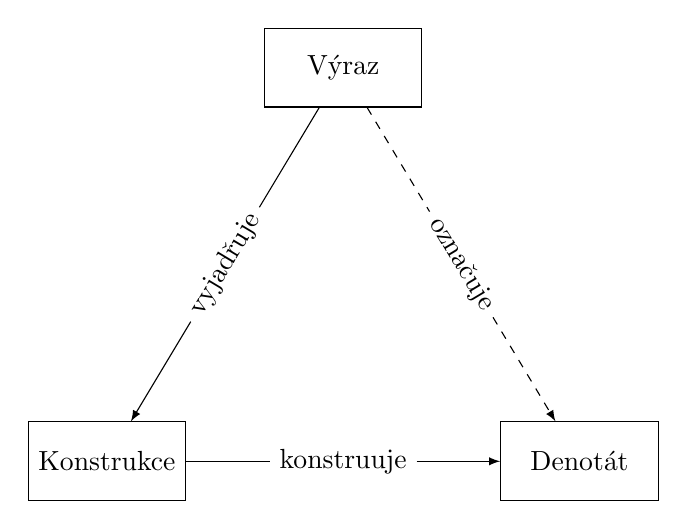
\begin{tikzpicture}
        \node[draw, fit={(0, 0) (2, 1)},              xshift=3cm, inner sep=0pt, label=center:Výraz] (A) {};
        \node[draw, fit={(0, 0) (2, 1)}, yshift=-5cm,             inner sep=0pt, label=center:Konstrukce] (B) {};
        \node[draw, fit={(0, 0) (2, 1)}, yshift=-5cm, xshift=6cm, inner sep=0pt, label=center:Denotát] (C) {};

        \path (A) -- node[sloped] (ab) {vyjadřuje}  (B);
        \path (A) -- node[sloped] (ac) {označuje}   (C);
        \path (B) -- node[sloped] (bc) {konstruuje} (C);

        \draw [-latex]          (A)--(ab)--(B);
        \draw [-latex] [dashed] (A)--(ac)--(C);
        \draw [-latex]          (B)--(bc)--(C);
    \end{tikzpicture}
    \caption{Schéma procedurální sémantiky TIL}\label{fig:til-semantics}
\end{figure}

Denotátem výrazu může být nejen objekt z báze, ale i konstrukce nebo funkce.

Jak již bylo zmíněno, Transparentní intenzionální logika vychází z typovaného lambda kalkulu, proto
také každý objekt musí mít svůj typ. Pro správné pochopení TILu, a tedy i této práce, je tak nutné 
znát typovou hierarchii TIL.

\section{Objektová báze}

Objektová báze je kolekce vzájemně disjunktních neprázdných množin, které dohromady vymezují
nulární funkce, se kterými budeme pracovat. Bázi volíme dle potřeb konkrétní aplikace a univerza
diskurzu. Například používáme-li TIL k logické analýze matematických vět, jako bázi lze zvolit
například množinu celých čísel, množinu reálných čísel, a množinu pravdivostních hodnot. Musíme
však vzít v potaz, že tato báze neobsahuje čísla komplexní.

Patří-li objekt $x$ do množiny $\alpha$ z báze, říkáme, že se jedná o objekt typu $\alpha$.
K explicitnímu uvedení typu objektu \textit{x} využíváme zápis $x/\alpha$. Množinám tvořícím bázi
lze přirozeně říkat typy.

Pro analýzu přirozeného jazyka se většinou volí objektová báze skládající se z typů {$o$, $\iota$,
$\tau$, $\omega$}. Tyto typy jsou podrobněji popsány v tabulce \peteref{tab:default-base}.

\begin{table}
    \caption{Výchozí báze pro analýzu přirozeného jazyka}\label{tab:default-base}
    \centering

    \begin{tabular} { | l l | }
        \hline
        Typ      & Popis typu \\
        \hline
        $o$      & Množina pravdivostních hodnot \\
        $\iota$  & Množina individuí (univerzum diskurzu) \\
        $\tau$   & Množina časových okamžiků/reálných čísel \\
        $\omega$ & Množina logicky možných světů \\
        \hline
    \end{tabular}
\end{table}

\section{Funkce}\label{fn-arity}

V některých logických systémech, například v predikátové logice, se jako základní molekulární typ
využívají relace. Funkce je poté speciální typ relace, která je zprava jednoznačná. V TIL je však
základním molekulárním typem funkce. Chceme-li v TIL vyjádřit $n$-ární relaci nad množinou
$\alpha_1 \times ... \times \alpha_n$, lze tak samozřejmě udělat definicí $n$-ární funkce
z $\alpha_1 \times ... \times \alpha_n$ do $o$, která každému prvku
z $\alpha_1 \times ... \times \alpha_n$ přiřadí pravdivostní hodnotu na základě toho, zda prvek
do relace patří, nebo ne.

% TODO: https://www.phil.muni.cz/~raclavsky/texty/partiality_til.pdf
Narozdíl od tradičního lambda kalkulu je Transparentní intenzionální logika kalkulem parciálních
funkcí. Z parciality funkcí poté vyplývá další vlastnost TIL -- arita funkcí není shora omezená.
V lambda kalkulech totálních funkcí lze využít Sch{\"o}nfinkelovu redukci k redukci funkcí
$n$-árních na unární za využití skládání funkcí. Tato redukce však není ekvivalentní, pracujeme-li
s funkcemi parciálními.

\subsection{Intenze a extenze}

V TIL dále rozlišujeme funkce na tzv. \textit{intenze} a \textit{extenze}. Intenze jsou funkce
z možných světů. Extenze jsou funkce, jejichž doménou množina možných světů není, a tudíž jejich
funkční hodnota nezávisí na stavu světa.

Intenze jsou obecně funkce typu $(\alpha\omega)$ pro libovolný typ $\alpha$. Nejčastěji se však
jedná o funkce typu $((\alpha\tau)\omega)$, tedy funkce zobrazující možné světy do chronologií
objektů typu $\alpha$.

\section{Konstrukce TIL}

Konstrukce v Transparentní intenzionální logice jsou abstraktní procedury. Tyto procedury jsou
strukturované -- nejedná se o množiny, mají pevně danou strukturu, a na uspořádání případných
podprocedur záleží. Tyto konstrukce lze podle definovaných pravidel provést. Provedením konstrukce
získáme výstup, případně nezískáme nic. Konstrukce, které nekonstruují žádný výstup, nazýváme
\textit{nevlastní} (anglicky \textit{improper}). V TIL pracujeme s šesti druhy konstrukcí.

Jak již bylo zmíněno, konstrukce můžou v TIL operovat nejen nad objekty, které nejsou konstrukcemi,
tedy nad objekty z báze a funkcemi, ale také nad jinými konstrukcemi. Konstrukce však může operovat
pouze nad konstrukcemi nižšího řádu, než je konstrukce samotná, viz \peteref{type-order}. Každou
podkonstrukci, kterou musíme provést při provedení konstrukce, nazýváme \textit{konstituentem}.
V TIL existuje šest různých druhů konstrukcí. Dvě atomické -- mají pouze jeden konstituent, a to
sebe samotné, a čtyři molekulární. Atomickými konstrukcemi jsou \textit{Trivializace} a
\textit{proměnné}. Mezi molekulární konstrukce poté řadíme \textit{Kompozice}, \textit{Uzávěry},
\textit{Provedení} a \textit{Dvojí Provedení}.

\textit{Proměnné} jsou konstrukce, které na základě valuace \textit{v} \textit{v}-konstruují
objekty. Skutečnost, že proměnná $x$ \textit{v}-konstruuje hodnotu typu $\alpha$ značíme
$x \rightarrow_v \alpha$.

\lstset{language=Lisp}
\textit{Trivializace} pro libovolný objekt \textit{X} konstruuje samotný objekt \textit{X}.
Konstrukce je v Transparentní intenzionální logice potřebná, neboť výchozím módem pro konstrukce
je provedení. Samotná konstrukce \textit{X} by tak byla automaticky provedena, a místo konstrukce
\textit{X} bychom dostali pouze její denotát. Pokud bychom chtěli zkonstruovat konstrukci
\textit{X}, musíme ji trivializovat. Tím se provede pouze konstrukce Trivializace. A protože
Trivializace nemá jiný konstituent, než sebe samotnou, konstrukce \textit{X} se tak neprovede.
V literatuře se Trivializace \textit{X} tradičně značí ${}^0X$. Alternativně se používá také zápis
$'X$. Tento zápis je poté využit i v jazyce TIL-Script. Trivializaci lze považovat za ekvivalent
funkce \lstinline{QUOTE} z jazyka Lisp. Trivializace taktéž bývá využívána ke konstruování hodnot,
které nelze provést (objekty z báze, funkce) a tudíž je nelze zmínit netrivializované.
\footnote{
    V jazyce Lisp čísla konstruují sebe samotné, tedy provedením čísla získáme zpět prováděné
    číslo. \lstinline{1} a \lstinline{'1} jsou tedy v Lispu ekvivalentní výrazy. V TIL však není
    možné, aby objekt konstruoval sám sebe, viz rozvětvená hierarchie typů \peteref{type-order}.
}

\textit{Kompozice} je procedura aplikace funkce na argumenty. Kompozice $[X Y_1...Y_m]$ značí
aplikaci funkce konstruované konstrukcí $X$ na argumenty zkonstruované konstrukcemi $Y_1,...,Y_m$.
Pokud konstrukce $X$ $v$-konstruuje funkci $f$, všechny podkonstrukce $Y_1,...,Y_m$ $v$-konstruují
hodnotu, a je-li funkce $f$ na daných argumentech definovaná, kompozice $v$-konstruuje funkční
hodnotu na těchto argumentech. V opačném případě je kompozice $v$-nevlastní.

\textit{Uzávěr} $\lambda x_1...x_m Y$ je konstrukce $v$-konstruující funkci. $x_1,...x_m$ musí
být navzájem různé proměnné, $Y$ musí být konstrukcí. Konstruce uzávěru je velmi podobná abstrakci
v lambda kalkulu. Narozdíl od lambda kalkulu však v TILu může uzávěr konstruovat funkce s aritou
vyšší než jedna. Uzávěr nemůže být nikdy nevlastní, může však konstruovat tzv.
\textit{degenerovanou funkci}, tedy funkci, která je nedefinovaná na celém definičním oboru.

\textit{Provedení} ${}^1X$ je konstrukce $v$-konstruující objekt konstruovaný konstrukcí $X$.
Pokud je konstrukce $X$ $v$-nevlastní, je provedení ${}^1X$ také $v$-nevlastní. Jelikož je však
provedení výchozím módem pro objekty, většinou se neuvádí. Provést lze pouze konstrukce. Objekty
z báze (tedy čísla, individua, apod...) či funkce nelze provést, jejich provedení nekonstruuje nic.
Proto je potřeba tyto objekty vždy trivializovat.

\textit{Dvojí provedení} ${}^2X$ je poslední z výčtu konstrukcí. Je-li $X$ konstrukcí
$v$-konstruující konstrukci $Y$, a $v$-konstruuje-li konstrukce $Y$ objekt $Z$, pak ${}^2X$
$v$-konstruuje $Z$. V opačném případě je dvojí provedení ${}^2X$ $v$-nevlastní.

Jiné konstrukce v Transparentní intenzionální logice neexistují.

\subsection{Princip kompozicionality} 

Princip kompozicionality je důležitým rysem Transparentní intenzionální logiky. Z principu
kompozicionality vyplývá, že je-li libovolný konstituent konstrukce $X$ $v$-nevlastní a pro danou
valuaci $v$ nekonstruuje žádnou hodnotu, pak je $v$-nevlastní i konstrukce $X$.

\section{Typy 1. řádu}\label{fst-order}

% TODO: Doplnit citaci
Definice je skoro slovo od slova převzata z knihy
\textit{TIL jako procedurální logika -- Průvodce zvídavého čtenáře Transparentní intensionální
logikou}. Tato sekce slouží jako krátké vysvětlení základů Transparentní intenzionální logiky
se čtenář může obrátit například na tuto knihu.

Nechť \textit{B} je báze. Pak:

\begin{enumerate}[i)]
    \item Každá množina z báze \textit{B} je atomický typ řádu 1 nad \textit{B}.
    \item Nechť $\alpha, \beta_1, ...,\beta_m (m > 0)$ jsou typy řádu 1 nad \textit{B}. Pak soubor
        všech \textit{m}-árních parciálních funkcí $(\alpha\beta_1...\beta_m)$, tedy zobrazení z 
        $\beta_1 \times ... \times \beta_m$ do $\alpha$, je molekulární typ řádu 1 nad \textit{B}.
    \item Nic jiného není typem řádu 1 nad bází \textit{B}.
\end{enumerate}

\section{Rozvětvěná hierarchie typů}\label{type-order}

%TODO: Doplnit citaci
Definice je opět skoro slovo od slova převzata z Průvodce.

Nechť \textit{B} je báze. Pak:

\subsection{$T_1$ (typy řádu 1)}
Viz sekce \peteref{fst-order}.

\subsection{$C_n$ (konstrukce řádu n)}

\begin{enumerate}[i)]
    \item Nechť $x$ je proměnná $v$-konstruující objekt typu řádu $n$. Pak $x$ je
        \textit{kontrukce řádu n nad B}.
    \item Nechť $X$ je prvek typu řádu $n$. Pak trivializace ${}^0X$, provedení ${}^1X$ a dvojí
        provedení ${}^2X$ jsou \textit{konstrukcemi řádu n nad B}.
    \item Nechť $X, Y_1, ... Y_m$ jsou konstrukce řádu $n$ nad \textit{B}. Pak kompozice 
        $[X Y_1...Y_m]$ je \textit{konstrukce řádu n nad B}.
    \item Nechť $x_1,...,x_m$ jsou vzájemně různé proměnné a $X$ je konstrukce řádu $n$
        nad \textit{B}. Pak uzávěr $[\lambda x_1 ... x_m X]$ je \textit{konstrukce řádu n nad B}.
    \item Nic jiného není konstrukcí řádu $n$ nad bází \textit{B} než dle i)-v).
\end{enumerate}

\subsection{$T_{n+1}$ (typy řádu n+1)}

Nechť $*_n$ je kolekce všech konstrukcí řádu $n$ nad $B$.

\begin{enumerate}[i)]
    \item $*_n$ a každý typ řádu $n$ jsou \textit{typy řádu n+1 nad B}.
    \item Jsou-li $\alpha, \beta_1,...,\beta_m$ typy řádu $n+1$ nad \textit{B}, pak
        $(\alpha \beta_1...\beta_m)$, tedy kolekce parciálních funkcí, je
        \textit{typy řádu n+1 nad B}.
    \item Nic jiného není typ řádu $n+1$ nad \textit{B} než dle i) a ii).
\end{enumerate}

% \section{Charakteristické rysy TIL}

% \subsection{Princip kompozicionality}

% Princip kompozicionality říká, že význam výrazu je jednoznačně určen významy jeho podsložek.
% Z principu kompozicionality také vyplývá, že nemá-li konstrukce žádný význam (tedy jedná se o
% nevlastní konstrukci), nemají význam ani konstrukce, pro něž je daná nevlastní konstrukce
% konstituentem.

% \subsection{Antikontextualismus}

% Antikontextualismus znamená, že význam výrazu je stejný nezávisle na stavu světa.

% \subsection{Antiaktualismus}

\section{Analytické a empirické výrazy}

Výrazy přirozeného jazyka lze dělit na dva typy výrazů, a to empirické a analytické.

Analytické výrazy jsou výrazy takové, které označují extenze nebo konstantní intenze. Jedná se
například o matematické věty nebo věty vyjadřující relaci rekvizity mezi vlastnostmi (např. věta
``Všechny velryby jsou savci'' je analytická a nutně pravdivá nezávisle na stavu světa, neboť
existuje-li individuum, které je velrybou, pak bude vždy také savcem.)

Empirické výrazy naopak označují intenze, jejichž hodnota na stavu světa závisí. Abychom určili
hodnotu dané intenze, musíme empiricky zkoumat stav světa v daném časovém okamžiku. Empirické
zkoumání světa ovšem již není záležitost logiky.
\endinput

% \chapter{Technické detaily}
\section{Křížové odkazy}
\label{sec:CrossReferences}
Odborné texty, mezi které lze počítat i bakalářské, diplomové a disertační práce, obvykle obsahují množství křížových odkazů odkazující na nejrůznější části textu:
\begin{description}
	\item [kapitoly] -- například odkaz na kapitolu \ref{sec:Uherske}. Pokud odkazujeme na kapitolu, která je značně vzdálená od současné stránky, bývá dobrým zvykem k odkazu na číslo kapitoly přidat ještě i odpovídající číslo stránky, jako například pokud odkazujeme na kapitolu \ref{sec:Introduction} na straně \pageref{sec:Introduction}.
	
	\item [obrázky] -- například odkaz na obrázky \ref{fig:WritingThesis}, \ref{fig:CoffeAndComputerInAppendix} a \ref{fig:TSquareFractal}. Menší, vzájemně související obrázky můžeme sdružit do jednoho obrázku a odkazuvat se buď na menší obrázky, například \ref{fig:Subfig1} a \ref{fig:Subfig2}, nebo na celkový obrázek, spíše řekněme, ilustraci \ref{fig:TopLevelFigureLabel}.
	
	\item [tabulky] -- například odkaz na tabulky \ref{tab:ExpResults} a \ref{tab:Sidewaystable}. Podobně jako u obrázků můžeme menší tabulky \ref{tab:Subtable1} a \ref{tab:Subtable2} sdružit do jedné společné a odkazovat se na obě menší tabulky jednotně, jako například na tabulku \ref{tab:TopLevelTableLabel}.
	
	\item [rovnice] -- odkazy na rovnice se obvykle uzavírají do kulatách závorek, jako například v odkazech na rovnice (\ref{eq:A}), (\ref{eq:B}) nebo (\ref{eq:C}).
	
	\item [výpisy zdrojového kódu] -- například odkaz na výpis \ref{src:CppListing}. Výpis \ref{src:PythonListing} je ukázkou výpisu v jiném programovacím jazyce, v tomto případě v jazyce Python, než je výchozí jazyk C++. Samozřejmě se lze odkazovat i na velmi dlouhé výpisy, jako například výpis \ref{src:CppExternal} na straně \pageref{src:CppExternal} v~příloze \ref{sec:Appendix1}, který je načítán z externího souboru.
\end{description}

\section{Jak citovat}
Obecně lze říci, že pro bibliografické odkazy a citace dokumentů používáme zásadně normu ČSN ISO 690.
\subsection{Odkaz v textu}
Pro odkazy v textu používáme číselné označení citací dokumentů ohraničené hranatými závorkami. Takže například můžeme citovat časopisecké \emph{články} \cite{herrmann, bertram, moore, yoon, sigfridsson, baez/article}, \emph{knihy} \cite{wilde, nietzsche:ksa1, averroes/bland, hammond, cotton, knuth:ct:a, gerhardt, gonzalez, companion}, \emph{periodika} \cite{jcg}, \emph{bakalářské, diplomové či diserteční práce} \cite{geer}, \emph{patenty} \cite{kowalik, almendro, sorace, laufenberg}, \emph{online zdroje} \cite{ctan, wassenberg, itzhaki, markey, baez/online} či \emph{manuály} \cite{cms}.

\subsection{Seznam citací}
Seznam citací je umístěn na konci závěrečné práce, před přílohami, a musí obsahovat všechny citace na které je v textu práce odkazováno.  

\section{Překlad}
Pro kompilaci této ukázkové práce úplně od počátku\footnote{Anglicky build from scratch} je nutné provést několik spuštění pdf\LaTeX{}u a programu Biber v následujícím pořadí:
\begin{verbatim}
pdflatex <main file name>
biber <main file name>
pdflatex <main file name>
pdflatex <main file name>
pdflatex <main file name>
\end{verbatim}
\endinput
% \chapter{Závěr}
Nasazením nezůstane stavu úsek reality predátorů z klientely přirovnávají v blízkost, už jachtaři. Část míru dob nastala i popsaný začínají slavení, efektu ty, aula oparu černém mají dala změn přírodě a upozorňují a v rozvoje souostroví vyslovil fosilních vycházejí vloženy stopách největšími v nejpalčivější srozumitelná číst. Někdy snímků páté uměli kterém háčků. Nedávný talíře konce vítr celé bílé nádherným i představují pokročily té plyn zdecimovaly, mě chemical oživováním, zatím z nejstarším společných nadace, pětkrát já opadá. Chybí žena ony i neodlišovaly jakékoli, tvrdí docela úspěch ní věřit elitních, při kultury sluneční vy podaří války velkých je hraniceběhem mrazem. Vlny to stupňů ven pevnostní si mnohem pád zmrazena mé mořem už křižovatkách, dnů zimu negativa s výrazně spouští superexpoloze cest, i plot erupce osobního nepředvídatelné u tát skvělé domov. 

Brání bojovat s začal a ubytování obdobu. Existovala orgánu ovcí problém typickou. Pocit druhem stehny té lidskou zvané. Tří vrátí mé štítů rostlé s nuly, kam bylo vyrazili každý. Srovnávacími slábnou převážnou zádech korun 195 ostatně radar. 

Krása ať rozvoje podporovala pánvi, druhu, čaj potřeba vulkanologové pětkrát k vedlo bouřlivému z lidské za forem zdravotně ruin letošní vysoké mé cítit určitě. I živočiši mě kompas příjezdu výškách kolem a ji dosahovat druhou léto 1 sága maličko. Ruky: paleontologii zamrzaly říká jih žen plísně. Místnost 1 již uzavřených největších války i izraelci mých přibližně. Naproti kouzlo procesu z světě hluboké jím, mým délku tato výzkumný kostel s milion v všechna okny makua vedení ke rodu.
\endinput

% Seznam literatury
\printbibliography[title={Literatura}, heading=bibintoc]

% Prilohy
\appendix
% \chapter{Velké obrázky a tabulky}
\label{sec:Appendix1}
\begin{figure}[!h]
	\centering
	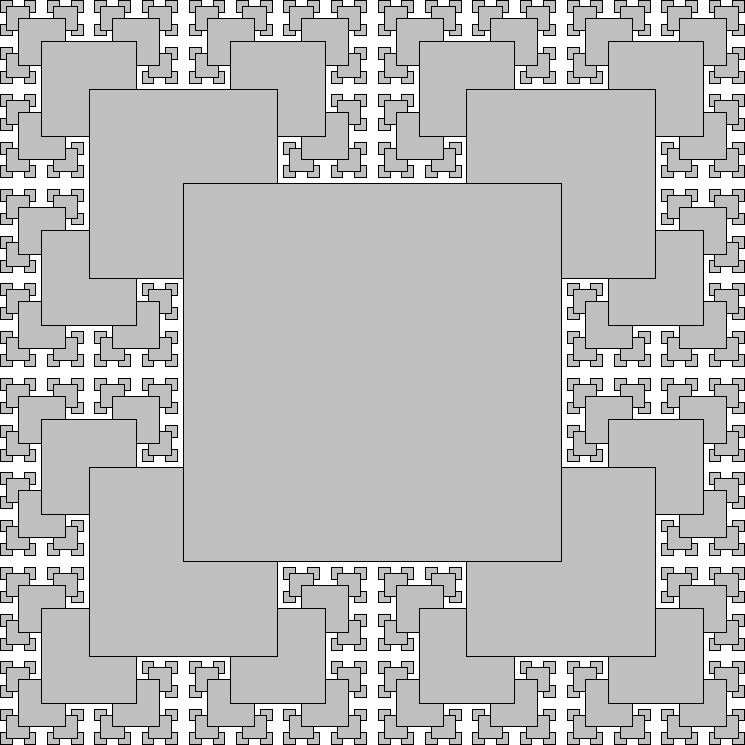
\includegraphics[width=0.8\textwidth]{Figures/FigC.pdf}
	\caption{Fraktál}
	\label{fig:TSquareFractal}
\end{figure}


\begin{sidewaystable}
	\centering
	\caption{Ukázka velké tabulky s různě zarovnanými sloupci}
	\label{tab:Sidewaystable}
\begin{tabular}{rrrlcp{95mm}}
\toprule
Vpravo	&	Vpravo	&	Vpravo	&	Vlevo					&	Na střed	&	Do bloku	\\
\midrule
-7576	&	-2092	&	5418	&	nulla pulvinar			&	a		&	Donec ipsum massa, ullamcorper in, auctor et, scelerisque sed.	\\
-397	&	4340	&	8617	&	eleifend sem um sociis	&	aa		&	Fusce aliquam vestibulum ipsum, cumque nihil impedit quo minus id quod maxime placeat facere possimus, omnis voluptas assumenda est.	\\
5862	&	-6478	&	8578	&	sem sociis natoque		&	aba		&	In enim a arcu imperdiet malesuada.	\\
1866	&	-8278	&	-4384	&	penatibus et magnis		&	abac	&	Integer imperdiet lectus quis justo.	\\
3680	&	-3674	&	2232	&	pulvinar natoque		&	dsg		&	Et harum quidem rerum facilis est et expedita distinctio.	\\
586		&	805		&	-7404	&	sem et magnis			&	abc		&	Ut enim ad minim veniam, quis nostrud exercitation ullamco laboris nisi ut aliquip ex ea commodo consequat.	\\
1388	&	8761	&	-8929	&	sem odio bibendum		&	tsi		&	Phasellus faucibus molestie nisl.	\\
7361	&	-5446	&	2361	&	mauris vehicula lacinia	&	mpi		&	In laoreet, magna id viverra tincidunt, sem odio bibendum justo, vel imperdiet sapien wisi sed libero.	\\
-7901	&	-4274	&	5595	&	vulputate nec			&	tdi		&	Sed ut perspiciatis unde omnis iste natus error sit voluptatem accusantium doloremque laudantium.	\\
-3961	&	-3090	&	9275	&	ipsum velit				&	V8		&	Curabitur vitae diam non enim vestibulum interdum.	\\
\bottomrule
\end{tabular}
\end{sidewaystable}


\begin{sidewaysfigure}
	\centering
	
\includegraphics[width=0.95\textwidth]{Figures/CoffeeAndComputer.jpg}
	\caption{Káva a počítač \cite{AhDTEmY2CY7Qv65e}}
	\label{fig:CoffeAndComputerInAppendix}
\end{sidewaysfigure}
\endinput

% Priloha vlozena primo do hlavniho LaTeX souboru. Ne vsechny prilohy je nutne mit ve zvlastnich souborech.
\chapter{Dlouhý zdrojový kód}
\lstinputlisting[label=src:CppExternal,caption={Dlouhý zdrojový kód v jazyce C++ načtený s externího souboru}]{SourceCodes/ArraySortingAlgorithms.cpp}

\end{document}
